\pdfoutput=1
\documentclass[11pt]{article}
\usepackage[review]{acl}
\usepackage{times}
\usepackage{latexsym}
\usepackage[T1]{fontenc}
\usepackage[utf8]{inputenc}
\usepackage{microtype}
\usepackage{inconsolata}
\usepackage{graphicx}
\usepackage{booktabs}
\usepackage{amsmath}
\usepackage{xcolor}
\usepackage{colortbl}
\definecolor{hblue}{HTML}{2A78D6}
\definecolor{horange}{HTML}{EB6834}
\definecolor{tier}{HTML}{EEF4FC}
\definecolor{muted}{HTML}{8A8984}

\newcommand{\eqh}[1]{\mathrm{EQ}_{#1}}

\title{Told to Look Further Ahead, Language Models Change Their Moves\\but Not Their Scores: A Controlled Test of Lookahead}

\author{Anonymous ACL submission}

\begin{document}
\maketitle

\begin{abstract}
Ask a language model for the move that pays off eight steps from now, and it may give you the move that pays off right away. Existing planning benchmarks cannot tell these apart, because they change the problem whenever they change the horizon. We built a test that holds everything fixed except the stated horizon. Each item is a frozen state from a turn-based card game. Between prompts, only the number of decisions ahead at which the goal is measured changes. Exhaustive search gives the provably best move for every horizon, and the scoring gives no credit for ignoring the instruction. Across eight open models from four families, only the two largest reasoning models change their choices in the right direction. Even they mostly trade the greedy move for a different wrong move. Only about one in three of their changed answers is the best long-horizon move, and their scores do not improve. Models without explicit reasoning ignore the horizon altogether, including a 70-billion-parameter model. An exact rulebook or hidden card names leave this picture unchanged. Thinking longer, in short, is not the same as planning further. The test needs only a deterministic simulator, so it carries over to any domain that has one. We release the states, the exact answers and every model response.
\end{abstract}

\section{Introduction}

Planning means accepting a worse result now for a better one later. A chess player gives up a pawn to open a file. A card player spends a turn weakening an opponent before attacking. Language models now act as agents that are expected to plan in this sense. Their instructions often say so directly: think ahead, consider the long run, optimize over the next several steps. Whether a model actually changes its decision when told to look further ahead is a basic question. Current benchmarks cannot answer it.

The difficulty is that the horizon is rarely the only thing that changes. Planning benchmarks pose problems whose length varies together with their content \citep{valmeekam2023planbench,zheng2024naturalplan,xie2024travelplanner}. Game benchmarks score a whole episode, which mixes rule knowledge, tactics and luck into one number \citep{costarelli2024gamebench,paglieri2025balrog,park2025orak}. When a model does worse on a longer task, we cannot tell whether it failed to look ahead or whether the longer task was simply harder. A clean answer needs the same problem posed twice, with only the horizon changed, and a ground truth for each version.

This paper provides that test. Each item is one frozen state from a deterministic, turn-based card game. We ask a model for its next move under a goal measured after $H$ decisions, for $H \in \{1,2,4,8\}$. Everything else stays identical: the state, the legal moves, the scoring rule and the answer format. Exhaustive search over the game's simulator gives the exact value of every legal move at every horizon. Figure~\ref{fig:example} shows a state from the test. A quick attack wins if the goal is one decision away. A setup move that makes every later hit land harder wins if the goal is eight decisions away.

Two design choices make the test hard to fool. First, a model that ignores the horizon scores exactly zero on our main measure. We judge its long-horizon and short-horizon answers by the same long-horizon standard, so only a changed answer can earn credit. Second, half of the states are controls, where the best move is the same at every horizon. A model that merely reacts to a longer instruction moves its answers on both kinds of state. A model that uses the horizon moves them only where the horizon matters.

We chose a card game because it is a rare domain where all of this is possible at once. Short-term and long-term moves come apart naturally. The full state fits in about a thousand tokens of text. A simulator can be copied and searched exactly. The game is also an established testbed for language agents \citep{bateni2024language,park2025orak}.

We test eight open-weight models from four families. Three findings stand out.
\begin{itemize}
\item \textbf{Only large reasoning models respond to the horizon.} Qwen3-32B and gpt-oss-120b choose the long-horizon move more often when told to look eight decisions ahead. Smaller models and models without explicit reasoning do not, including a 70-billion-parameter model.
\item \textbf{Responding is not planning.} The responsive models give up the greedy move, but only about one time in three do they replace it with the correct long-horizon move. On control states they also abandon moves that were already right, so their scores do not improve.
\item \textbf{The pattern is not about knowing the game.} A pre-registered test that supplies an exact rulebook leaves the picture unchanged, and so does a second test that replaces every card and enemy name with a code.
\end{itemize}

We make three contributions. The first is a controlled-horizon benchmark of 1,760 game states with an exact answer key at four horizons. The second is a protocol for building such benchmarks in any domain with a simulator, including scoring that a model cannot game by ignoring the instruction. The third is evidence that current models treat ``look further ahead'' as a cue to avoid the obvious answer, without optimizing for the horizon they were given. All analyses were frozen before the models ran, and every amendment is versioned. We release the states, the exact action values, the prompts and every model response.

\begin{figure}[t]
\centering
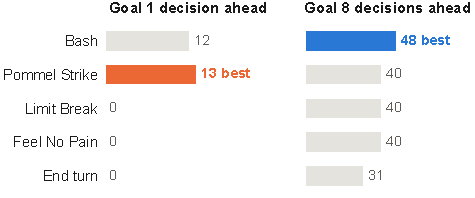
\includegraphics[width=\columnwidth]{figures/example.pdf}
\caption{One state from the benchmark (Ironclad against the Slime Boss, 2 energy). The boss is \emph{Vulnerable}, taking 50\% more damage, for one more turn. Bars give the exact value of each legal move, found by exhaustive search. With a one-decision goal, Pommel Strike deals the most damage now. With an eight-decision goal, Bash is best. It deals slightly less now but extends Vulnerable, so the attacks of the next turns keep their bonus. The state, the moves and the scoring rule are identical in both prompts. Only $H$ changes.}
\label{fig:example}
\end{figure}

\section{The Game in One Page}
\label{sec:game}

The test is built on \emph{Slay the Spire}, a single-player card game. No knowledge of the game is needed to follow this paper. Table~\ref{tab:glossary} defines every game term we use.

\paragraph{How a fight works.} The player fights one or more enemies. Each turn the player draws cards and has 3 energy to spend. Every card costs energy and does one thing: deal damage, gain \emph{block} that absorbs damage, or apply an effect that changes later turns. When the player ends the turn, each enemy acts. Enemies announce their next move in advance, so the player can see an attack coming. The fight ends when one side runs out of health.

\paragraph{Why it is a planning problem.} Many cards pay off later. \emph{Vulnerable} makes an enemy take 50\% more damage for several turns, so applying it first and attacking afterwards beats attacking twice. Poison deals damage every turn rather than at once. Block spent now can save more health than damage dealt now. A player who only maximizes the next move plays a different game from a player who looks ahead, and the difference is measurable.

\paragraph{Why a reimplementation.} We use a Python reimplementation of the game's combat with seeded random streams. Our oracle copies the state and searches every line of play, up to two million positions per state and horizon. The commercial game cannot do this, because it runs on the Java virtual machine behind a modding interface with no cheap state copying. The reimplementation gives exact replay, a license-clean release and fully reproducible states. Our question does not require an exact copy of the commercial game. It asks whether a model uses the horizon under rules it has been given. In one condition every prompt states our rules in full, and the results do not change (Section~\ref{sec:results}). Appendix~\ref{app:engine} lists where its rules differ from the commercial game.

\begin{table}[t]
\centering
\small
\setlength{\tabcolsep}{4pt}
\begin{tabular}{@{}p{0.29\columnwidth}p{0.64\columnwidth}@{}}
\toprule
Term & Meaning \\
\midrule
Card & One action the player can take, at a cost in energy \\
Energy & Budget per turn (3), lost if unspent \\
Hand, draw pile & Cards playable now, and cards still to come in a known order \\
Block & A shield that absorbs damage until the owner's next turn \\
Intent & The enemy's announced next move, e.g.\ ``attack for 12'' \\
Strength & Each point adds 1 damage to every hit \\
Vulnerable & The target takes 50\% more attack damage \\
Weak & The attacker deals 25\% less attack damage \\
Poison & The target loses that much health each turn, then 1 less \\
Ironclad, Silent & The two playable characters, with different cards \\
\midrule
Decision & One choice: play one card, or end the turn \\
Horizon $H$ & How many decisions ahead the goal is measured \\
Oracle & Exhaustive search giving the exact value of every move \\
Sensitive state & No move is best at both $H{=}1$ and $H{=}8$ \\
Control state & Some move is best at both $H{=}1$ and $H{=}8$ (ties count) \\
\bottomrule
\end{tabular}
\caption{Game and protocol terms. The lower block is ours.}
\label{tab:glossary}
\end{table}

\section{The Controlled-Horizon Protocol}
\label{sec:protocol}

\paragraph{States.} We generate fights from fixed random seeds against five boss and elite encounters. Each fight advances by a short scripted prefix and is then frozen as a \emph{state}. Every state uses its own seed, so states are independent draws. A model never saw a state before the analysis plan was frozen. From the audited pool we release 1,760 states, 880 per character. Half of each character's states are \emph{sensitive}: the best move at $H{=}1$ and the best move at $H{=}8$ do not overlap. The other half are \emph{controls}, where some move is best at both horizons. The two sets are similar in encounter mix, number of legal moves, hand size, energy and health (Appendix~\ref{app:props}).

\paragraph{Prompt.} The model sees the full state as JSON: its health, energy, hand, the enemy's health and intent, every pile in its exact order and the remaining combat counters. It is told to choose ``the next action that maximizes the stated utility after exactly $H$ decision transitions.'' Utility is damage dealt minus health lost, plus 1,000 for a win and minus 1,000 for a loss. A decision is one card play or the end of a turn, so $H{=}8$ spans about two turns. We therefore test multi-turn lookahead within a fight. Payoffs that arrive after decision $H$ count for nothing, by design. A model that plays for the whole fight can therefore lose credit on some states. This is why the prompt states the horizon, the utility and the counting rule exactly, and a variant that defines ``decision transition'' explicitly changes nothing (Appendix~\ref{app:amendments}). It answers with one action in JSON. The prompts for different $H$ differ in that one number and nothing else, which we verify byte for byte.

\paragraph{Oracle.} For each state and horizon, depth-limited exhaustive search over the simulator returns the exact value $v_H(a)$ of every legal first action $a$. This value assumes best play for the remaining $H-1$ decisions. We score an answer by its normalized value
\[
\eqh{H}(a) = \frac{v_H(a) - \min_{a'} v_H(a')}{\max_{a'} v_H(a') - \min_{a'} v_H(a')},
\]
which is 1 for a best move and 0 for the worst. Illegal, unparseable or truncated answers score 0.

\paragraph{The main measure.} Let $a_1$ and $a_8$ be a model's answers to the same state at $H{=}1$ and $H{=}8$. The model's gain from the instruction is
\[
g = \eqh{8}(a_8) - \eqh{8}(a_1),
\]
both answers judged by the eight-decision standard. A model that ignores $H$ gives the same answer twice and earns $g{=}0$ on every state. Real gains come from changing the answer for the better. Our primary statistic is the difference between the mean $g$ on sensitive states and on control states. It is positive only if the model gains more where the horizon matters than where it does not. We test it per character with a 10,000-sample bootstrap over states at $\alpha = 0.025$, which keeps the two-character family at 0.05.

\paragraph{Lookahead use.} We also count how often the $H{=}8$ answer is a best eight-decision move on sensitive states. We compare that rate with an \emph{H-blind baseline}: the same rate for the model's own $H{=}1$ answer. A model that ignores $H$ matches its baseline exactly, and McNemar's exact test \citep{mcnemar1947} compares the two. We also report the \emph{greedy rate}, the share of answers that are best only at $H{=}1$.

\paragraph{Validity gates.} A model's run counts as confirmatory only if two conditions hold. First, at most 1\% of its answers were cut off by the 16,000-token output limit. Second, at most 2\% of states lost an answer to an execution failure. Runs that fail a gate are reported but do not enter any confirmatory test.

\paragraph{Pre-registration.} The states, prompts, scoring code, gates and analysis plan were frozen and fingerprinted before any model was run. Adding a model, a condition or a serving flag required a versioned amendment that may only add, never change. Appendix~\ref{app:amendments} lists every amendment. Analyses not in the frozen plan are labeled post hoc.

\section{Models and Setup}
\label{sec:setup}

We test eight open-weight models from four families (Table~\ref{tab:models}). Four reason explicitly before answering: Qwen3 at 8B, 14B and 32B parameters with thinking enabled \citep{yang2025qwen3}, and gpt-oss-120b \citep{openai2025gptoss}. Four answer directly: Llama-3.1-8B and Llama-3.3-70B \citep{dubey2024llama}, Mistral-7B \citep{jiang2023mistral} and Qwen2.5-7B \citep{qwen2025qwen25}. Open weights let us pin every model to an exact revision and serving stack, so every number in this paper can be regenerated.

All models are served with vLLM \citep{kwon2023vllm} and decoded greedily (temperature 0, fixed seed) with a 16,000-token output budget in a 32,768-token context. Each model answers all 1,760 states at all four horizons, 7,040 queries, in a counterbalanced order. No query is ever retried. A query lost to an infrastructure failure is recorded as a failure.

\begin{table}[t]
\centering
\small
\setlength{\tabcolsep}{3.5pt}
\begin{tabular}{@{}llcc@{}}
\toprule
Model & Family & Reasons & Weights \\
\midrule
Mistral-7B-Instruct-v0.3 & Mistral & no & BF16 \\
Qwen2.5-7B-Instruct & Qwen & no & BF16 \\
Llama-3.1-8B-Instruct & Llama & no & BF16 \\
Llama-3.3-70B-Instruct & Llama & no & FP8 \\
Qwen3-8B & Qwen & yes & BF16 \\
Qwen3-14B & Qwen & yes & BF16 \\
Qwen3-32B & Qwen & yes & BF16 \\
gpt-oss-120b & OpenAI & yes & MXFP4 \\
\bottomrule
\end{tabular}
\caption{Models. MXFP4 is gpt-oss's released precision. FP8 lets the 70B model fit two GPUs. Revisions and serving stacks are pinned in Appendix~\ref{app:amendments}.}
\label{tab:models}
\end{table}

\section{Results}
\label{sec:results}

Seven of the eight runs pass both validity gates. Qwen3-8B cut off 4.0\% of its answers at the token limit, so its numbers are descriptive only.

\subsection{Only large reasoning models respond to the horizon}

Figure~\ref{fig:use} shows, for each model, how often its answer is a best eight-decision move on sensitive states, next to its H-blind baseline. For six of the eight models the two numbers coincide. Telling them to look eight decisions ahead does not move their answers toward the long-horizon move. This holds at every horizon we tested (Appendix~\ref{app:curves}). Qwen3-32B and gpt-oss-120b are the exceptions. On both characters, their $H{=}8$ answers hit the long-horizon move far more often than their own $H{=}1$ answers do. For gpt-oss the rates are .36 against .25 (Ironclad) and .31 against .21 (Silent). For Qwen3-32B they are .28 against .22 and .30 against .19. McNemar's test gives $p \le .026$ in all four cases.

Size alone does not produce this. Llama-3.3-70B has more than twice the parameters of Qwen3-32B and no explicit reasoning, and its use rate sits at its baseline on both characters. Within one family the effect grows with scale: Qwen3-8B does not respond, Qwen3-14B moves slightly but stays within its baseline, and Qwen3-32B responds clearly.

\begin{figure}[t]
\centering
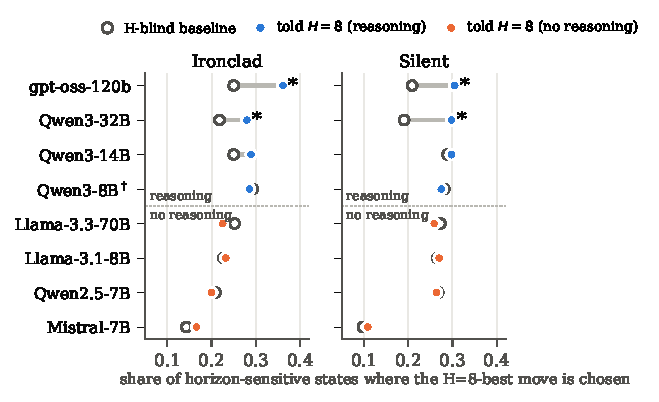
\includegraphics[width=\columnwidth]{figures/use_vs_baseline.pdf}
\caption{How often each model picks the best eight-decision move on sensitive states when told $H{=}8$ (filled), against its H-blind baseline (open), which is its own $H{=}1$ answer judged by the same standard. A model that ignores $H$ sits on its baseline. $^*$McNemar $p<.05$. $^\dagger$Failed the truncation gate, so descriptive only.}
\label{fig:use}
\end{figure}

\subsection{Responding is not planning}

The primary statistic tells a more sobering story (Table~\ref{tab:primary}). Five models show no effect, with confidence intervals tight around zero. The three models that move their answers, Qwen3-14B, Qwen3-32B and gpt-oss-120b, show a positive difference on Ironclad and, for gpt-oss, on Silent. In every case the difference comes from the control side. Their gain on sensitive states is close to zero, while their score on control states \emph{falls} when told to look further ahead. The instruction makes them abandon moves that were already right.

Figure~\ref{fig:decomp} shows where the answers go (a post hoc breakdown). When gpt-oss is told $H{=}8$, it gives up the greedy move on 314 of the 880 sensitive states, yet only 91 of those switches land on a best long-horizon move. The rest go to other moves, which on average score no better than the greedy move they replaced. Qwen3-32B behaves the same way: 73 of 209 switches find the long-horizon move. On control states, both models drop between a fifth and a third of their correct answers. The instruction works as a cue to avoid the obvious move. It does not lead the models to the move that looking ahead would reveal.

The state in Figure~\ref{fig:example} shows the pattern in a single case. At $H{=}1$, gpt-oss plays Pommel Strike, the best move, and explains that it ``deals the most damage this turn.'' At $H{=}8$ it switches to Feel No Pain, a card that grants block whenever a card is later exhausted, reasoning that it ``sets up future block generation.'' The switch sounds like planning, but the move is worth .53 on the eight-decision scale. Bash, which keeps the boss Vulnerable, is worth 1. Qwen3-32B plays Bash at both horizons.

\begin{table}[t]
\centering
\footnotesize
\setlength{\tabcolsep}{2pt}
\begin{tabular}{@{}lrr@{}}
\toprule
Model & Ironclad & Silent \\
\midrule
Mistral-7B & $+.013$ {\scriptsize$[-.03,+.06]$} & $+.033$ {\scriptsize$[-.01,+.08]$} \\
Qwen2.5-7B & $-.001$ {\scriptsize$[-.01,+.01]$} & $-.014$ {\scriptsize$[-.03,+.00]$} \\
Llama-3.1-8B & $+.003$ {\scriptsize$[-.01,+.01]$} & $-.000$ {\scriptsize$[-.01,+.01]$} \\
Llama-3.3-70B & $+.016$ {\scriptsize$[-.03,+.06]$} & $+.001$ {\scriptsize$[-.04,+.04]$} \\
Qwen3-8B$^\dagger$ & $-.031$ {\scriptsize$[-.10,+.03]$} & $+.018$ {\scriptsize$[-.04,+.07]$} \\
Qwen3-14B & $\mathbf{+.100}$ {\scriptsize$[+.04,+.16]$} & $+.005$ {\scriptsize$[-.04,+.05]$} \\
Qwen3-32B & $\mathbf{+.125}$ {\scriptsize$[+.07,+.18]$} & $+.045$ {\scriptsize$[-.01,+.10]$} \\
gpt-oss-120b & $\mathbf{+.155}$ {\scriptsize$[+.09,+.22]$} & $\mathbf{+.074}$ {\scriptsize$[+.02,+.13]$} \\
\midrule
\multicolumn{3}{@{}l}{\footnotesize Of which, gain on sensitive / control states:} \\
gpt-oss-120b & $+.014 \,/\, {-.142}$ & $-.032 \,/\, {-.107}$ \\
\bottomrule
\end{tabular}
\caption{Primary statistic: gain from the $H{=}8$ instruction on sensitive states minus gain on control states, with 95\% bootstrap intervals. Bold: rejects zero at $\alpha=.025$. The lower row shows that the positive values come from losses on control states.}
\label{tab:primary}
\end{table}

\begin{figure}[t]
\centering
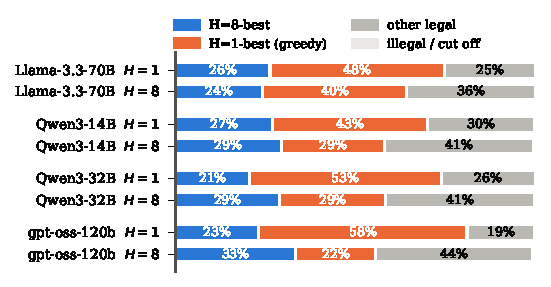
\includegraphics[width=\columnwidth]{figures/decomposition.pdf}
\caption{What models answer on sensitive states (both characters, 880 states) at $H{=}1$ and $H{=}8$. Responsive models move answers out of the greedy class, but mostly into other non-best moves. Post hoc.}
\label{fig:decomp}
\end{figure}

\subsection{It is not about knowing the game}

Our prompts name each card without describing it, so a model must recall what ``Bash'' does. A reviewer could fairly ask whether the horizon results reflect gaps in game knowledge, or recognition of famous card names, rather than planning. We tested both explanations in a pre-registered amendment on the 1,169 states that hold no targeted skill card (see Limitations). In the \emph{described} condition, every prompt carries an exact rulebook generated from the simulator: what each visible card does, how each enemy behaves and how every effect works. In the \emph{renamed} condition, every card, enemy and relic name, and the name of the game, is replaced by a neutral code such as ``Card K7''. We ran both conditions on one model that ignores the horizon (Llama-3.1-8B) and one that responds to it (gpt-oss-120b).

None of the eight pre-registered contrasts survives Holm correction \citep{holm1979} (Table~\ref{tab:knowledge}). With the rulebook, Llama-3.1-8B still ignores the horizon, with intervals of about $\pm.02$. Its blind spot is not a knowledge gap. gpt-oss plays somewhat better overall with the rulebook (mean $H{=}8$ quality rises from .71 to .76), but its use of the horizon does not change reliably. With all names hidden it still responds to the horizon at the same rate, so recognizing famous cards is not what drives it.\footnote{gpt-oss cut off 1.9\% of its renamed-condition answers, above the 1\% gate, so its familiarity contrasts are descriptive.}

\begin{table}[t]
\centering
\footnotesize
\setlength{\tabcolsep}{1.5pt}
\begin{tabular}{@{}llrr@{}}
\toprule
& & Knowledge & Familiarity \\
Model & Char. & {\scriptsize described $-$ base} & {\scriptsize renamed $-$ described} \\
\midrule
Llama-3.1-8B & IC & $-.003$ {\scriptsize$[-.02,+.02]$} & $+.017$ {\scriptsize$[-.02,+.05]$} \\
 & Silent & $-.000$ {\scriptsize$[-.02,+.02]$} & $-.005$ {\scriptsize$[-.04,+.03]$} \\
gpt-oss-120b & IC & $+.073$ {\scriptsize$[-.00,+.15]$} & $+.081^\dagger$ {\scriptsize$[-.00,+.16]$} \\
 & Silent & $+.073$ {\scriptsize$[-.01,+.15]$} & $+.084^\dagger$ {\scriptsize$[+.01,+.16]$} \\
\bottomrule
\end{tabular}
\caption{Knowledge and familiarity contrasts: change in the primary statistic between conditions, paired by state, 95\% intervals. None rejects after Holm correction over all eight. $^\dagger$Descriptive (gate failed).}
\label{tab:knowledge}
\end{table}

\subsection{Robustness}

Every conclusion above holds when any one of the five encounters is removed, and when the 591 states affected by the oracle limitation described under Limitations are removed (Appendix~\ref{app:robust}). A prompt variant that defines ``decision transition'' explicitly changes nothing for either model tested (Appendix~\ref{app:amendments}). The full-game scores of these models from an earlier version of the benchmark do not predict their horizon use. Those scores sit at a ceiling for combat and a floor for full runs, which is exactly why a controlled test is needed.

\section{A Recipe for Any Domain}
\label{sec:recipe}

Nothing in the protocol depends on cards. It needs four ingredients, and many domains supply all four.
\begin{enumerate}
\item \textbf{A deterministic simulator with copyable state}, so that every line of play can be replayed.
\item \textbf{An objective indexed by a horizon}, so that the same state has a best move for each $H$, found exactly or with a certified bound.
\item \textbf{Natural states where the horizon changes the answer}, selected without looking at any model, plus controls where it does not.
\item \textbf{Scoring that is invariant to ignoring $H$}: judge the short- and long-horizon answers by the same long-horizon standard, so a model gets credit only for changing its choice.
\end{enumerate}
Chess endgames come with tablebases that give exact values at every depth. Sokoban and other sliding puzzles have exact solvers. Inventory, scheduling and routing simulators trade cost now against cost later. Tool-using agents in a sandboxed environment can be scored after a fixed number of steps. In each case the same construction yields a controlled test of lookahead, with the same guard against a model scoring by ignoring the instruction. We built a 240-position chess pilot this way (Appendix~\ref{app:chess}). When told to look further ahead, gpt-oss-120b picks the best five-ply move more often, as in the card game. Unlike in the card game, it loses little where the short-horizon move was already right, and a post hoc rescoring without its truncated answers suggests a real gain. We release our generator, oracle and analysis code as a template for these extensions.

\section{Related Work}
\label{sec:related}

\paragraph{Planning benchmarks.} PlanBench checks plans exactly against symbolic domains \citep{valmeekam2023planbench}, and follow-up work finds that even reasoning models solve few of its harder instances \citep{valmeekam2024o1,kambhampati2024position}. NATURAL PLAN and TravelPlanner pose realistic planning tasks in natural language \citep{zheng2024naturalplan,xie2024travelplanner}. These benchmarks vary problem length together with problem content. We hold the problem fixed and vary only the horizon, which isolates whether a model uses it.

\paragraph{Games as agent benchmarks.} GameBench, BALROG, AgentBench and Orak evaluate agents across many games or environments and score episode outcomes \citep{costarelli2024gamebench,paglieri2025balrog,liu2024agentbench,park2025orak}. Such scores combine rule knowledge, tactics and long-range planning. Our test trades breadth for an exact answer key per horizon.

\paragraph{Language models and this game.} Bateni and Whitehead studied language-model play in a reimplementation of the same game and found that changing card names affects play \citep{bateni2024language}. Later work measured how well models judge card synergies \citep{kim2025synergy}, and Orak includes the commercial game in its suite \citep{park2025orak}. We use the game for a different purpose: as a source of states where a short and a long horizon disagree, with exact values for both. Our renaming condition extends their observation to horizon use.

\paragraph{Reasoning and lookahead.} Explicit intermediate reasoning improves many tasks \citep{wei2022cot}, and search over reasoning paths can help with problems that need lookahead \citep{yao2023tot}. Reasoning models are trained to think longer before answering \citep{deepseek2025r1,yang2025qwen3,openai2025gptoss}. Our results suggest that longer thinking makes a model respond to a stated horizon without making it optimize for that horizon.

\paragraph{Shortcuts.} Benchmarks can be solved by shortcuts that sidestep the intended skill \citep{geirhos2020shortcut}. Our scoring removes the shortcut of ignoring the instruction, and our control states separate real lookahead from a generic reaction to longer instructions.

\section{Conclusion}

We asked a simple question that existing benchmarks cannot answer: when told to look further ahead, does a language model choose differently, and better? With the state held fixed and an exact answer at every horizon, the answer for current open models is mostly no. Small and non-reasoning models ignore the horizon. Large reasoning models notice it and move away from the obvious move. They rarely find the move that lookahead would reveal, and they give up correct answers where the horizon does not matter. Training models to plan, and not merely to hesitate, will need tests that check the plan. The protocol here is one such test, and it transfers to any domain with a simulator.

\section*{Limitations}
\label{sec:limits}

\paragraph{One domain and open models.} All confirmatory states come from one game, and we test open-weight models up to 120B parameters. Closed frontier models may behave differently. The released states and scoring code make that test direct. A chess pilot (Appendix~\ref{app:chess}) covers two models and 240 positions and is descriptive only. One of the two models cannot play the positions, and gpt-oss exceeded the truncation gate. The pilot shows that the response to the horizon recurs in a second domain. It cannot settle whether the lack of an average gain does.

\paragraph{Simulator and oracle.} The reimplementation approximates the commercial game, and some rules differ (Appendix~\ref{app:engine}). The oracle values moves under our simulator's rules, which the prompt states in full in the described condition. The interface plays every non-attack card without a target, so seven targeted skill cards have no effect on enemies in the oracle. 591 states contain one. We therefore release the 1,169 unaffected states as the benchmark and list the 591 separately, flagged, for the record. Every main result holds on the clean states alone (Appendix~\ref{app:robust}), and the knowledge conditions use only those states. A corrected simulator would let the flagged states rejoin the benchmark.

\paragraph{Scope of the knowledge test.} The described and renamed conditions cover two models and the 1,169 unaffected states. gpt-oss exceeded the truncation gate in the renamed condition, so that contrast is descriptive.

\paragraph{Confounds between models.} Llama-3.1-8B and Llama-3.3-70B differ in post-training as well as size, and the 70B model runs in FP8. gpt-oss runs on a newer serving stack, which its architecture requires. Some runs used H200 rather than H100 GPUs. Greedy decoding gives one answer per query, and Qwen3's recommended settings use sampling. A sampled run would add variance estimates within each model. The answer-change analysis (Figure~\ref{fig:churn}), the chance and heuristic baselines and the robustness analyses were not pre-registered.


\bibliography{references}

\appendix
\section{Pre-registration, Amendments and Models}
\label{app:amendments}

The base protocol (states, prompts, scoring, gates, analysis) was frozen with a SHA-256 fingerprint before any model was run. Eight amendments followed, each frozen before the run it covers. Each may only add a model, a prompt condition or a serving flag.
\begin{enumerate}
\item Adds Llama-3.1-8B and DeepSeek-R1-Distill-Qwen-14B. The latter was excluded when only 2 of its first 8 answers fit in the 16,000-token budget.
\item Adds a prompt condition that defines ``decision transition'' explicitly. It made no significant difference for Llama-3.1-8B or Qwen3-14B.
\item Adds Mistral-7B, Qwen2.5-7B and Qwen3-32B, and the comparison with earlier full-game scores.
\item Adds Llama-3.3-70B in FP8 across two GPUs.
\item Adds gpt-oss-120b on its own serving stack (vLLM 0.10.2, Transformers 4.56.2), which its architecture requires.
\item Adds the described and renamed conditions on the 1,169 states without targeted skill cards.
\item Reruns Llama-3.3-70B with vLLM's custom all-reduce disabled. The first attempt crashed before producing any answer, and its records are kept but never analyzed.
\item Adds Qwen3-32B with thinking switched off, the same checkpoint with one changed request flag. It was frozen after the thinking-on results were known, so we report it as a post hoc test of mechanism.
\end{enumerate}
Fingerprints (first twelve hex digits): base \texttt{697011782709}, amendments 1 to 8 \texttt{bac116c3e1d7}, \texttt{eadf64f3cea0}, \texttt{6eb87256470c}, \texttt{899adb8313cb}, \texttt{6b212296a3dd}, \texttt{b7f44796ac19}, \texttt{eaa20e7d6a2b}, \texttt{33d68bddacce}. The release lets anyone recompute them from the frozen files. Every other model runs on vLLM 0.8.5.post1 with Transformers 4.51.3. Pinned revisions (first ten hex digits): Mistral-7B-Instruct-v0.3 \texttt{c170c708c4}, Qwen2.5-7B-Instruct \texttt{a09a35458c}, Llama-3.1-8B-Instruct \texttt{0e9e39f249}, Llama-3.3-70B-Instruct \texttt{6f6073b423}, Qwen3-8B \texttt{b968826d9c}, Qwen3-14B \texttt{40c069824f}, Qwen3-32B \texttt{9216db5781}, gpt-oss-120b \texttt{b5c939de8f}. Seven queries of Qwen3-32B were lost when a shared filesystem filled up mid-run. They are recorded as failures and never retried, which leaves the run well inside the 2\% gate.

\section{Lookahead Use at Every Horizon}
\label{app:curves}

\begin{table*}[t]
\centering
\small
\begin{tabular}{@{}lcccccc@{}}
\toprule
& \multicolumn{3}{c}{Ironclad} & \multicolumn{3}{c}{Silent} \\
\cmidrule(lr){2-4}\cmidrule(l){5-7}
Model & $H{=}2$ & $H{=}4$ & $H{=}8$ & $H{=}2$ & $H{=}4$ & $H{=}8$ \\
\midrule
Mistral-7B & .07/.07 & .11/.09 & .17/.14 & .06/.06 & .11/.09 & .11/.10 \\
Qwen2.5-7B & .15/.15 & .18/.19 & .20/.21 & .13/.14 & .22/.23 & .26/.27 \\
Llama-3.1-8B & .14/.15 & .22/.21 & .23/.23 & .13/.13 & .19/.20 & .27/.27 \\
Llama-3.3-70B & .17/.16 & .23/.27 & .23/.25 & .10/.07 & .27/.24 & .26/.27 \\
Qwen3-8B$^\dagger$ & .19/.18 & .23/.26 & .29/.29 & .13/.12 & .24/.27 & .28/.28 \\
Qwen3-14B & .18/.20 & .28/.27 & .29/.25 & .15/.14 & .26/.22 & .30/.29 \\
Qwen3-32B & .19/.13$^*$ & .25/.20 & .28/.22$^*$ & .12/.15 & .30/.23 & .30/.19$^*$ \\
gpt-oss-120b & .25/.15$^*$ & .29/.23 & .36/.25$^*$ & .20/.14 & .28/.18$^*$ & .30/.21$^*$ \\
\bottomrule
\end{tabular}
\caption{Use rate / H-blind baseline on states where the best move at $H$ differs from the best at $H{=}1$. $^*$Use above baseline, McNemar $p<.05$. $^\dagger$Failed the truncation gate.}
\label{tab:curves}
\end{table*}

Table~\ref{tab:curves} gives the use rate and the H-blind baseline at $H \in \{2,4,8\}$. No model without explicit reasoning, and neither of the two smaller Qwen3 models, exceeds its baseline at any horizon.

\section{Robustness}
\label{app:robust}

\begin{table*}[t]
\centering
\small
\begin{tabular}{@{}lcccccc@{}}
\toprule
& \multicolumn{3}{c}{Ironclad} & \multicolumn{3}{c}{Silent} \\
\cmidrule(lr){2-4}\cmidrule(l){5-7}
Model & all & leave-one-out range & w/o targeted & all & leave-one-out range & w/o targeted \\
\midrule
Mistral-7B & +0.013 & [-0.004, +0.030] & +0.019 & +0.033 & [+0.023, +0.042] & +0.051 \\
Qwen2.5-7B & -0.001 & [-0.008, +0.003] & +0.000 & -0.014 & [-0.018, -0.011] & -0.007 \\
Llama-3.1-8B & +0.003 & [-0.000, +0.006] & -0.001 & -0.000 & [-0.003, +0.002] & +0.003 \\
Llama-3.3-70B & +0.016 & [+0.007, +0.025] & +0.032 & +0.001 & [-0.011, +0.009] & -0.006 \\
Qwen3-8B$^\dagger$ & -0.031 & [-0.055, -0.002] & -0.044 & +0.018 & [-0.006, +0.036] & +0.001 \\
Qwen3-14B & +0.100 & [+0.084, +0.120] & +0.093 & +0.005 & [-0.007, +0.018] & +0.018 \\
Qwen3-32B & +0.125 & [+0.105, +0.151] & +0.127 & +0.045 & [+0.021, +0.057] & +0.054 \\
gpt-oss-120b & +0.155 & [+0.134, +0.172] & +0.144 & +0.074 & [+0.058, +0.089] & +0.078 \\
\bottomrule
\end{tabular}
\caption{Primary statistic on all states, its range when each of the five encounters is left out in turn, and its value without the 591 states holding a targeted skill card. Post hoc.}
\label{tab:robust}
\end{table*}

Table~\ref{tab:robust} reports two post hoc checks. Every state comes from one of five encounters, so we recompute the primary statistic leaving each encounter out in turn. We also drop the 591 states holding a targeted skill card, which the oracle treats as having no effect on enemies. No sign changes for any model with a confirmatory result, and every rejected effect stays well away from zero.

\section{Engine Differences from the Commercial Game}
\label{app:engine}

The simulator implements the game's combat rules for two characters and the encounters used here. It is not a bit-exact clone. Differences that touch these states include the following.
\begin{itemize}
\item Some card values differ: Fiend Fire deals 6 per exhausted card, and Flame Barrier gives 8 block.
\item Metallicize grants its block at the start of the next turn.
\item Played power cards return to the discard pile and can be played again.
\item Choices that the game leaves to the player inside a card (which card to discard or exhaust) are made automatically by a fixed rule.
\item Lagavulin wakes when the player's health drops below its maximum. Slime Boss and Hexaghost follow fixed move cycles.
\end{itemize}
The described condition states our simulator's rules exactly, and the knowledge results hold under it. A complete list ships with the code.

\section{Prompt}
\label{app:prompt}

The system prompt names the character and fixes the JSON answer format. The user prompt gives the state as JSON, followed by a full-observability block with every pile in order and the simulator counters. It ends with the only line that changes across horizons: ``Choose the next action that maximizes the stated utility after exactly $H$ decision transitions. Utility is enemy HP lost minus player HP lost, plus 1000 for a win and minus 1000 for a loss.'' The described condition inserts the effect reference immediately before that line. The renamed condition also replaces every proper name with a neutral code and rewrites the system prompt's first sentence as ``You are an expert player of a deterministic deck-building card game.'' Complete prompts for every condition are in the release.


\end{document}
